\section{Creazione del training set}
Il dataset in input è stato prodotto a seguito delle operazioni di data integration su tre dataset originari. Durante queste operazioni, gli attributi privi di informazioi rilevanti ai fini dell'addestramento di un modello di Machine Learning sono stati rimossi, ottenendo un dataset già pronto all'uso. Per dividere il dataset in train set e test set, è stata definita una funzione ad hoc che permette di dividere il dataset in 10 parti, usandone poi 9 per il trainset e la restante per il testset. Questa funzione si è rivelata fondamentale per l'operazione di 10-fold cross validation, in cui il modello viene addestrato e testato su porzioni differenti del dataset.

\section{Analisi esplorativa del training set}
\section{Modelli di Machine Learning utilizzati}
Al fine di avere una misura di riferimento per i modelli che saranno proposti successivamente, è stato prodotto un modello baseline, che si limita a rispondere sempre failed ad ogni sottomissione di un sample. La risposta risulta essere sempre failed in quanto, dall'analisi esplorativa dei dati effettuata in precedente, è emerso che il valore di etichettatura più frequente era prorpio il fallimento del progetto.\\
In Figura \ref{fig:baselineperformance} sono riporatte le misure di performance ottenute con questo modello a seguito dell'operazione di 10 fold cross validation; notiamo come accuratezza e precisione si uniformino alla distribuzione delle etichettature failed nel dataset, mentre la recall rimanga ovviamente fissa ad 1.\\
Le curve ROC associate a questo modello, ripotate in Figura \ref{fig:baselineROC}, restituiscono un valore della Area Under Curve (AUC) molto variabile: ciò è dovuto dalla diversa distribuzione dei sample con etichettatura failed all'interno dei testset prodotti dal porcesso di 10-fold cross validation.

\begin{figure}
	\centering
	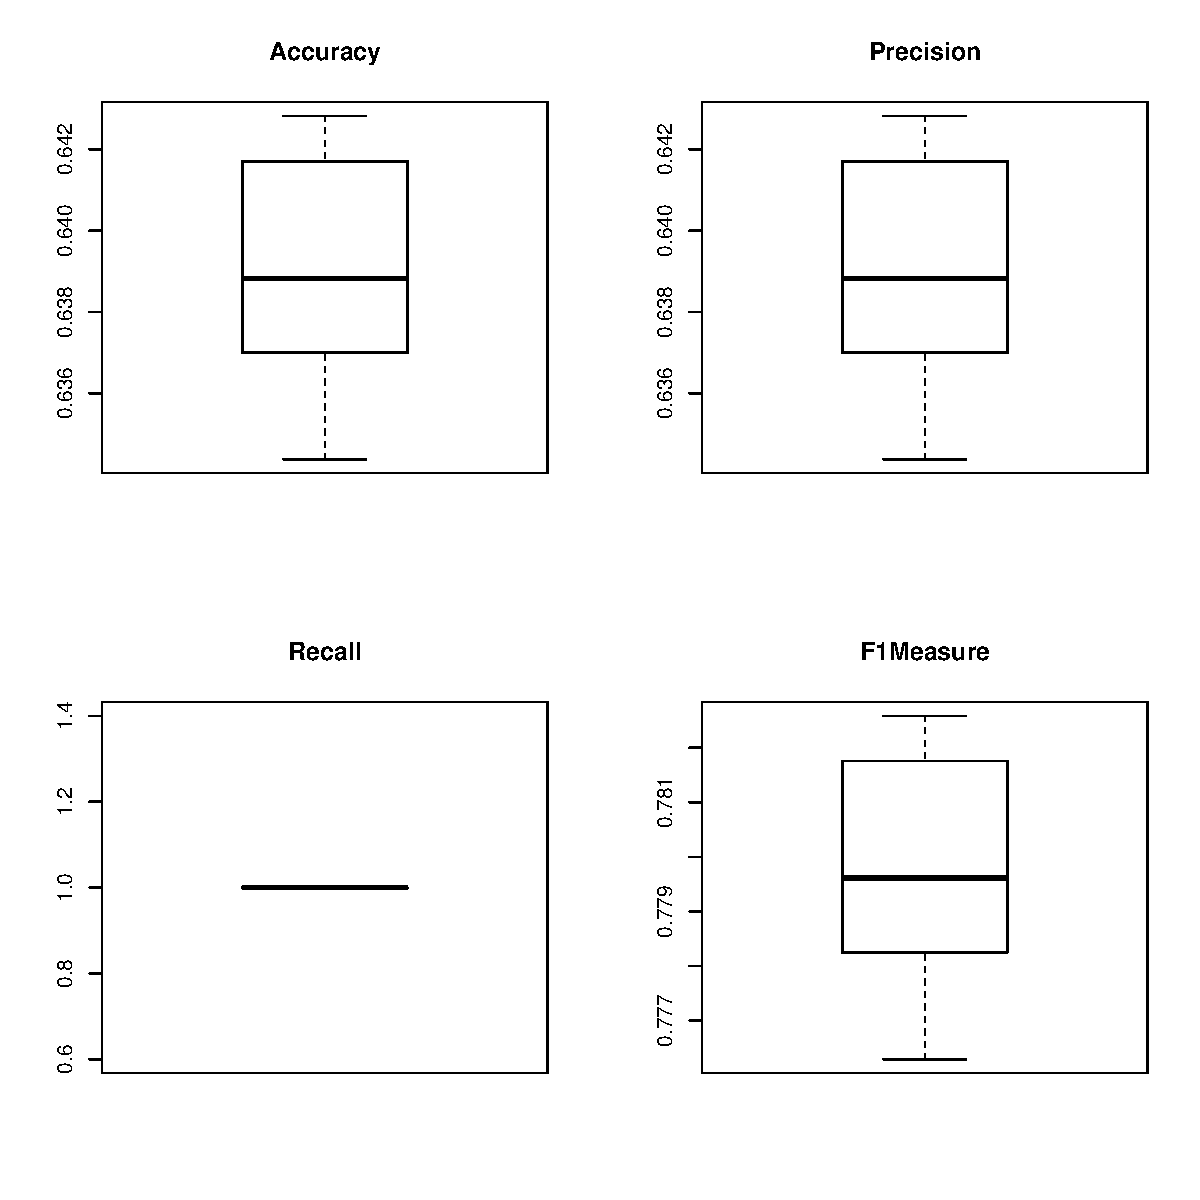
\includegraphics[width=0.7\linewidth]{../FinalResults/Baseline_performance}
	\caption[Boxplot relativi alle misure di perdormance del modello baseline.]{}
	\label{fig:baselineperformance}
\end{figure}

\begin{figure}
	\centering
	\subfloat{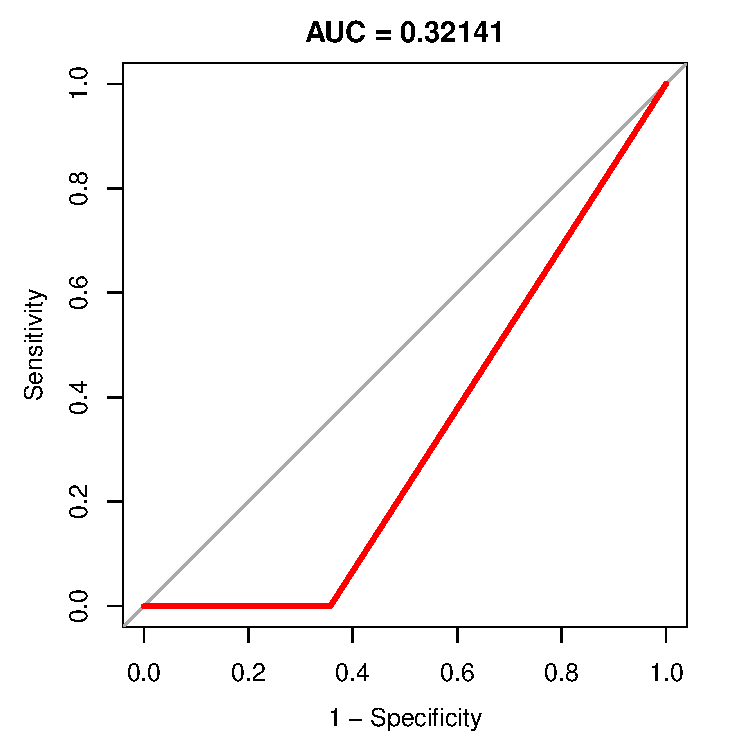
\includegraphics[width=0.3\linewidth]{../FinalResults/Images/baseline/auc_1.pdf}}\quad
	\subfloat{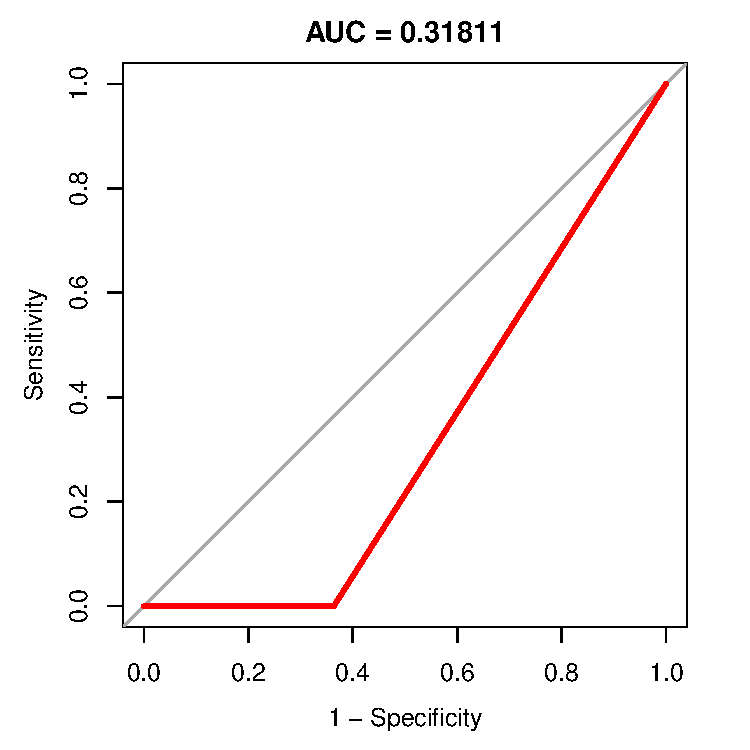
\includegraphics[width=0.3\linewidth]{../FinalResults/Images/baseline/auc_2.pdf}}\quad
	\subfloat{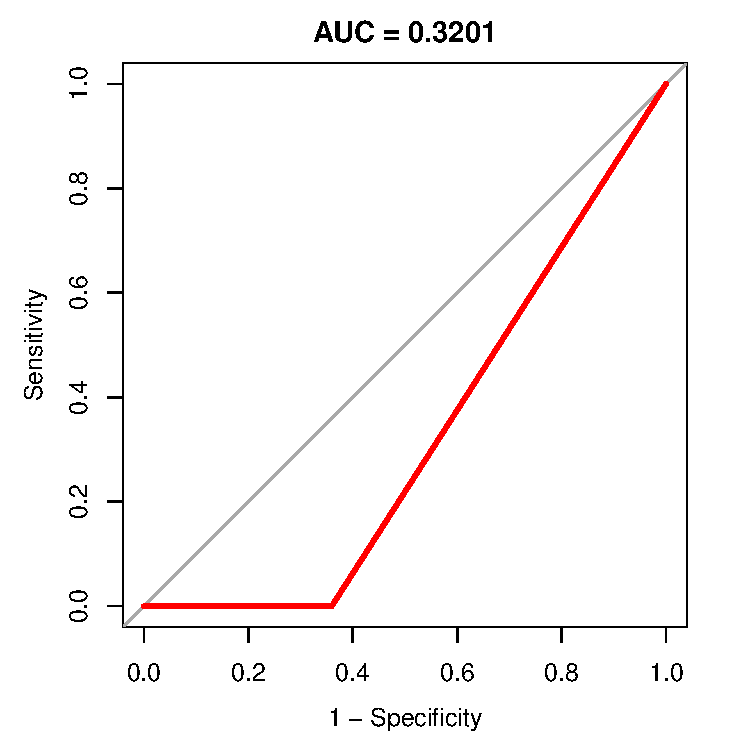
\includegraphics[width=0.3\linewidth]{../FinalResults/Images/baseline/auc_3.pdf}}\quad
	\subfloat{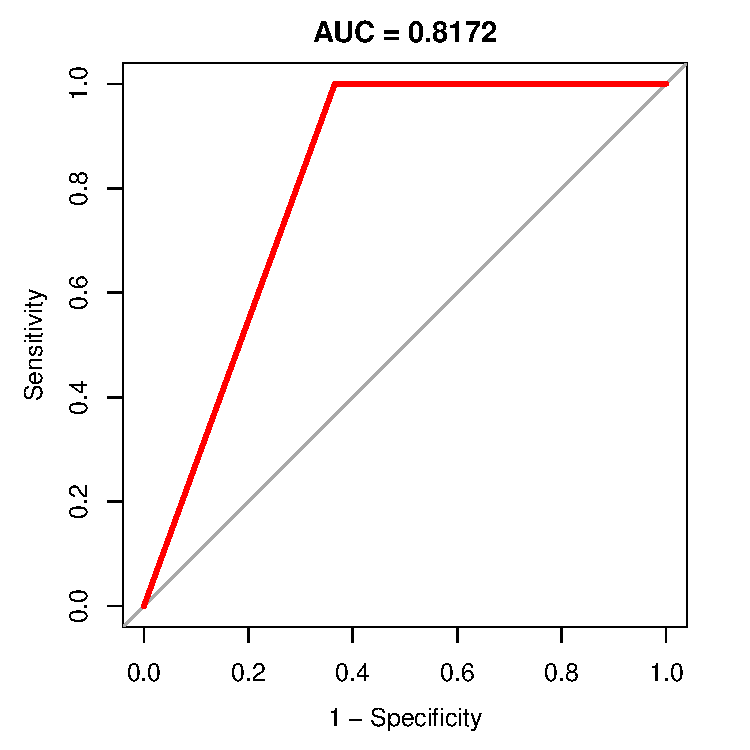
\includegraphics[width=0.3\linewidth]{../FinalResults/Images/baseline/auc_4.pdf}}\quad
	\subfloat{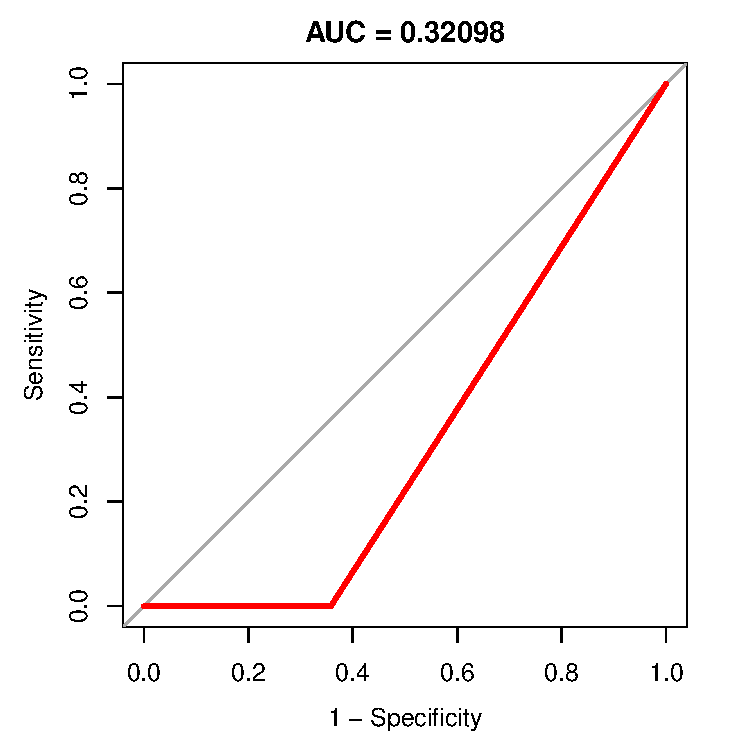
\includegraphics[width=0.3\linewidth]{../FinalResults/Images/baseline/auc_5.pdf}}\quad
	\subfloat{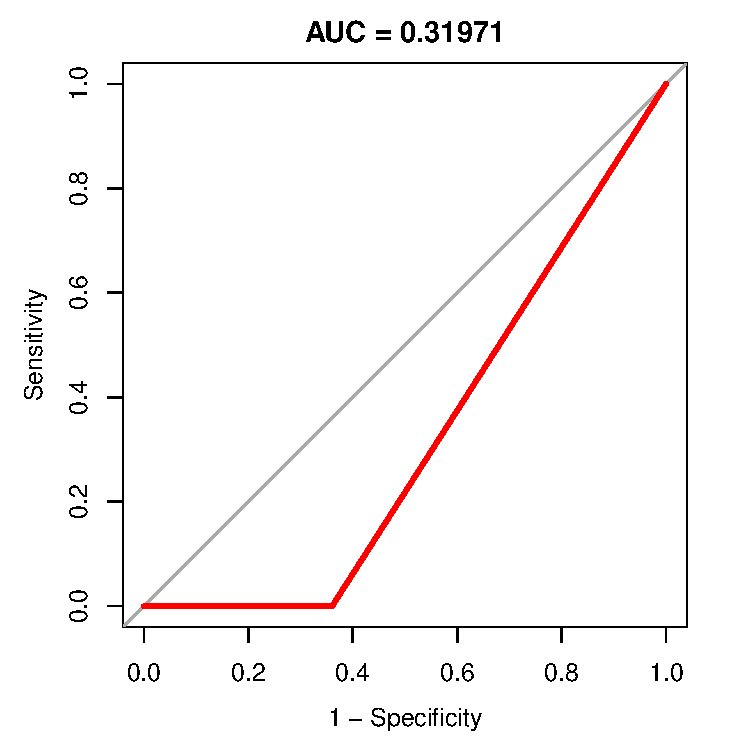
\includegraphics[width=0.3\linewidth]{../FinalResults/Images/baseline/auc_6.pdf}}\quad
	\subfloat{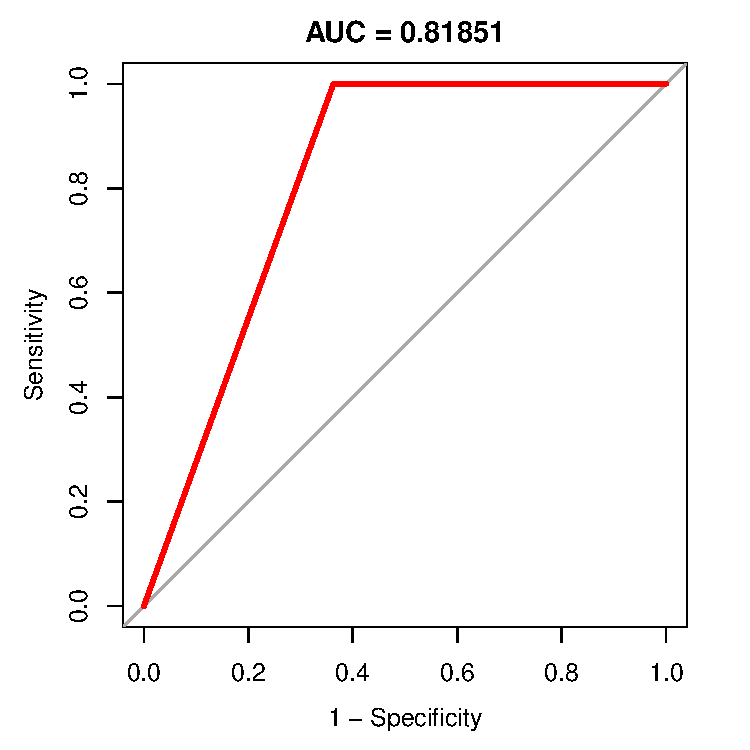
\includegraphics[width=0.3\linewidth]{../FinalResults/Images/baseline/auc_7.pdf}}\quad
	\subfloat{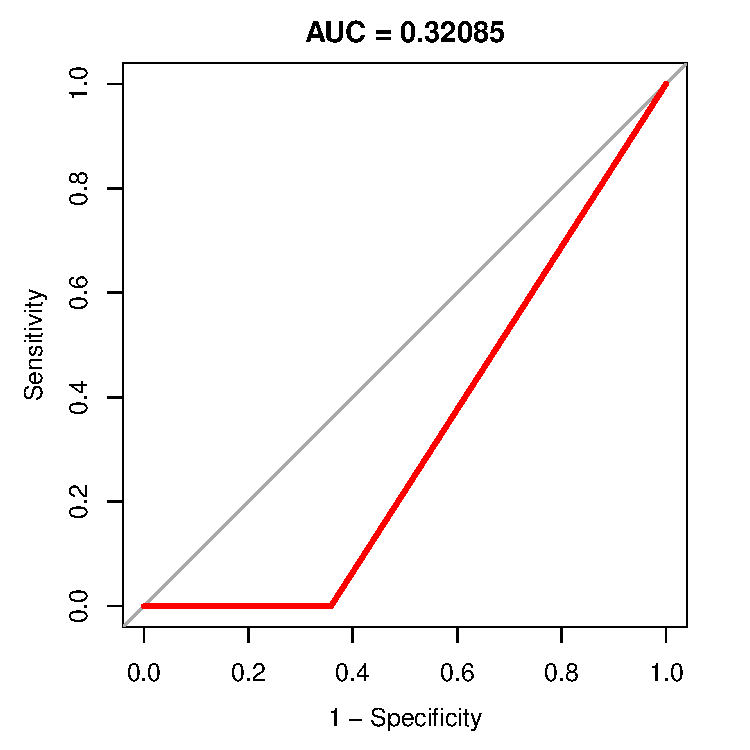
\includegraphics[width=0.3\linewidth]{../FinalResults/Images/baseline/auc_8.pdf}}\quad
	\subfloat{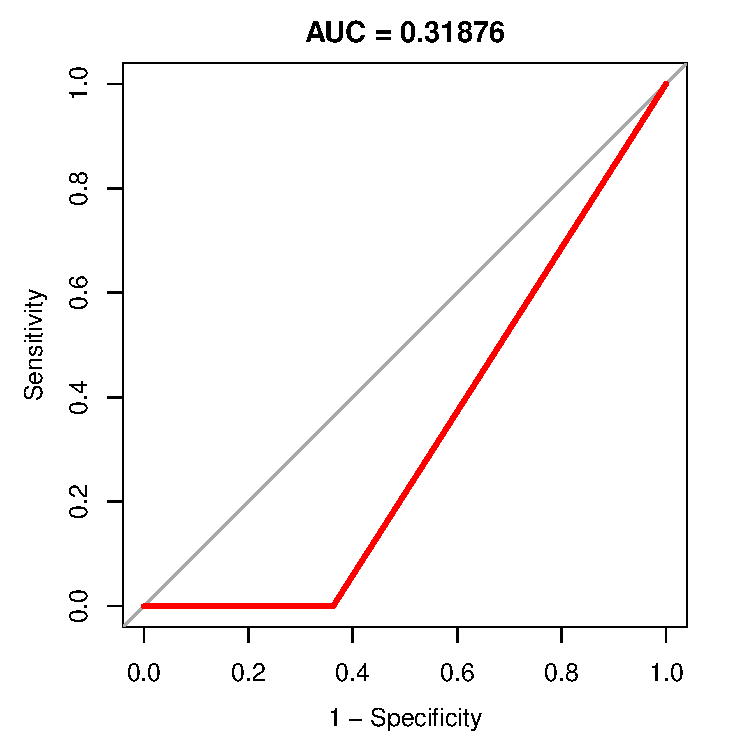
\includegraphics[width=0.3\linewidth]{../FinalResults/Images/baseline/auc_9.pdf}}\quad
	\subfloat{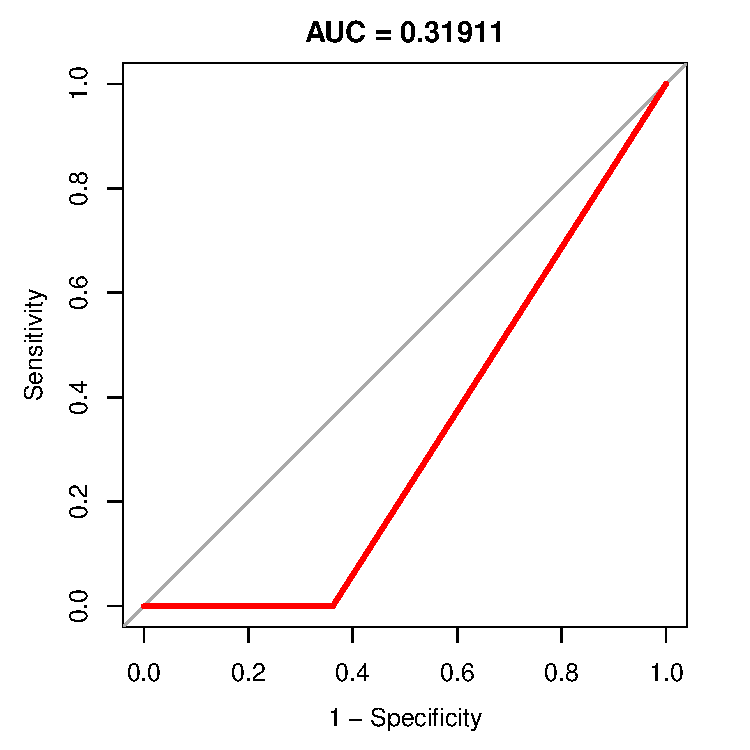
\includegraphics[width=0.3\linewidth]{../FinalResults/Images/baseline/auc_10.pdf}}\quad
	\caption{Curve ROC del modello baseline per la 10-fold cross validation.}
	\label{fig:baselineROC}
\end{figure}       

\subsection{Alberi decisionali}
\subsection{Reti neurali}
\subsection{Support Vector Machine}
\subsection{Naive Baies}